\section{Applications of {\fvgm}}\label{fvgm_sec:applications}
In this section, we apply {\fvgm} for verifying fairness-enhancing algorithms and depreciation attacks. We also demonstrate that {\fvgm} facilitates the computation of fairness influence functions by enabling the shift of bias from the original value due to individual features. 


\iffalse
\begin{figure}[t!]
	%\vspace{-1em}
	
	\centering
	\subfloat{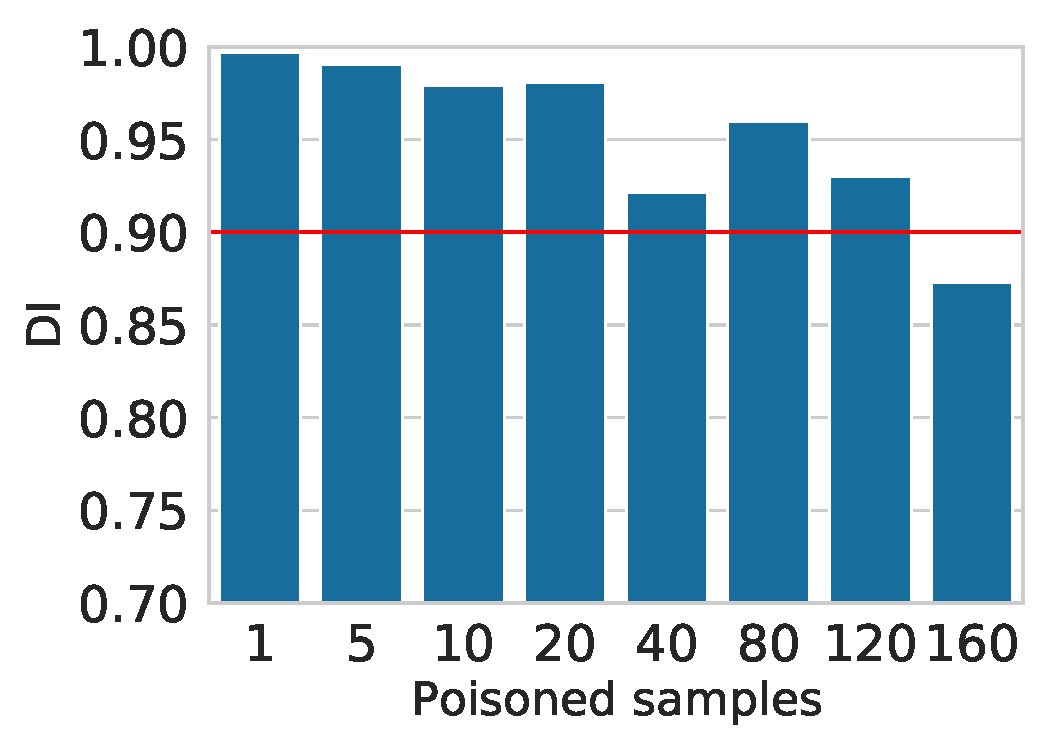
\includegraphics[scale=0.25]{figures/fairness/fvgm/disp_fairness_attack}}
	\subfloat{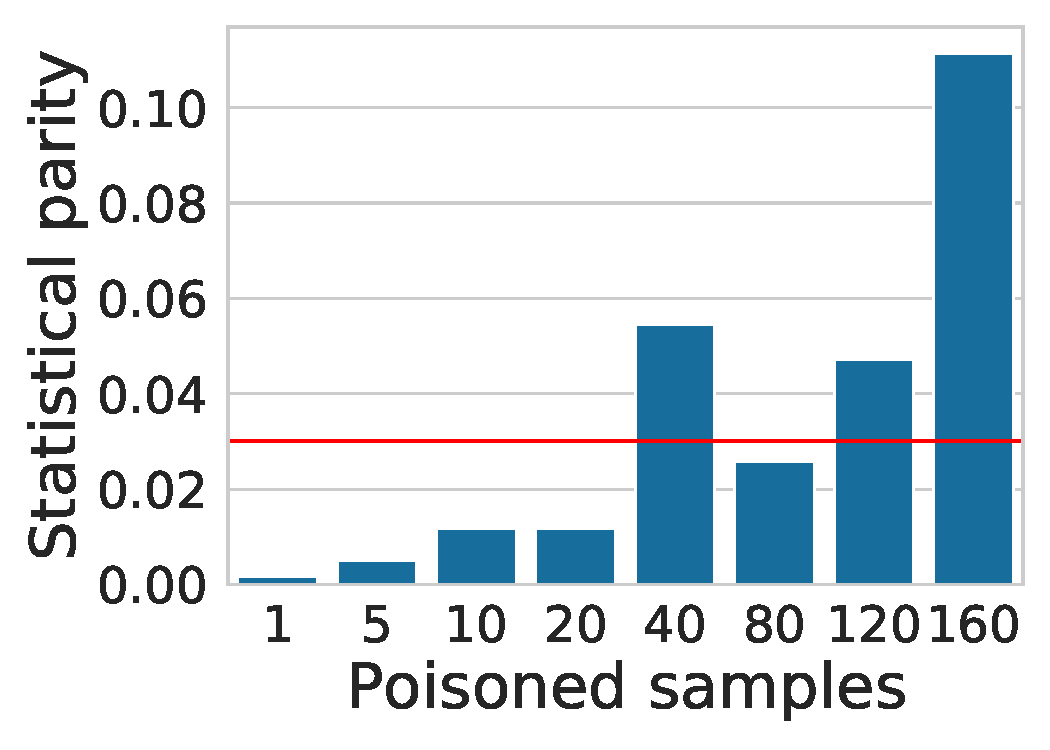
\includegraphics[scale=0.25]{figures/fairness/fvgm/stat_fairness_attack}}
	%\vspace{-0.5em}
	\caption{Verifying poisoning attack against fairness using {\fvgm}. The red line denotes the safety margin of the ML model against the attack.}\label{fvgm_fig:fairness_attacks}
\end{figure}
\fi


\paragraph{Verifying Fairness-enhancing Algorithms.} We deploy {\fvgm} in verifying the effectiveness of fairness-enhancing algorithms designed to ameliorate bias. For example, fairness 
pre-processing algorithms can be validated by applying {\fvgm} on the unprocessed and the processed data separately and comparing different fairness metrics. In Table~\ref{fvgm_tab:fair_algo_verification}, we report the effect of fairness algorithms w.r.t. four fairness metrics: disparate impact ($ \mathsf{DI} $), path-specific causal fairness ($ \mathsf{PCF} $), statistical parity ($ \mathsf{SP} $), and equalized odds ($ \mathsf{EO} $). Note that, fairness is improved if $ \mathsf{DI} $ increases and the rest of the metrics decrease. For instance, in most instances for Adult dataset, reweighing (RW)~\cite{kamiran2012data} and optimized pre-processing (OP)~\cite{calmon2017optimized} algorithms are successful in improving fairness. The exceptional case is the unfairness regarding the sensitive feature `sex', where OP algorithm fails in improving fairness metric $ \mathsf{EO} $. Thus, \textit{{\fvgm} verifies the enhancement and decrement in fairness by  fairness-enhancing algorithms. }



\begin{figure}
	\centering
	\subfloat{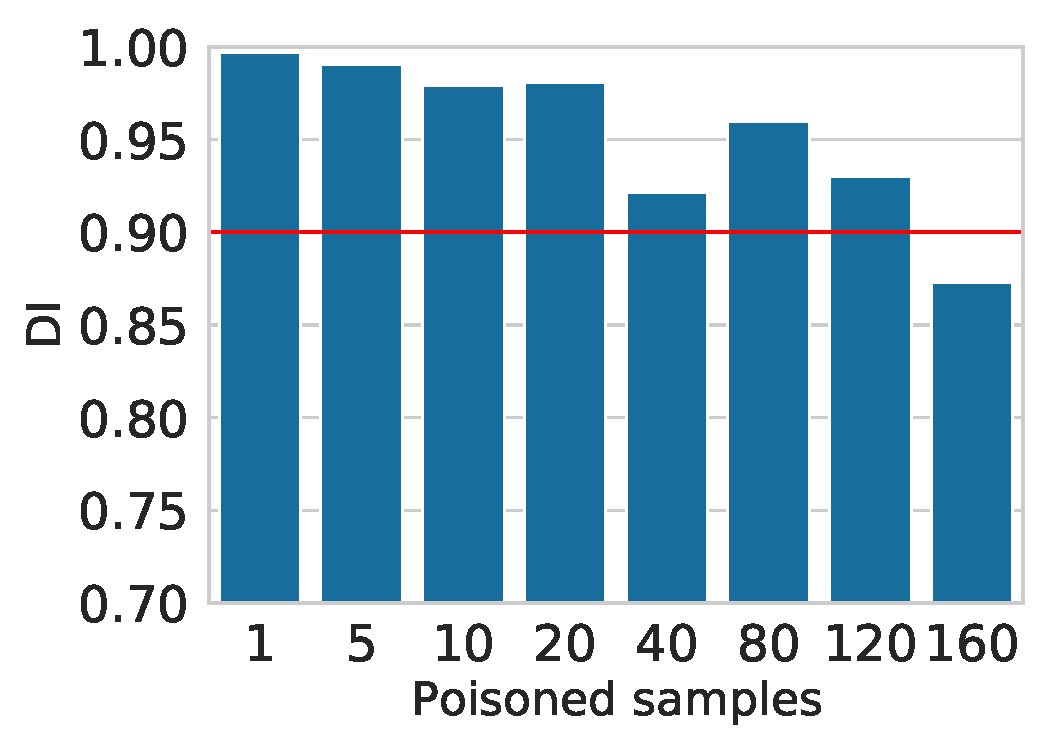
\includegraphics[scale=0.3]{figures/fairness/fvgm/disp_fairness_attack}}
	\subfloat{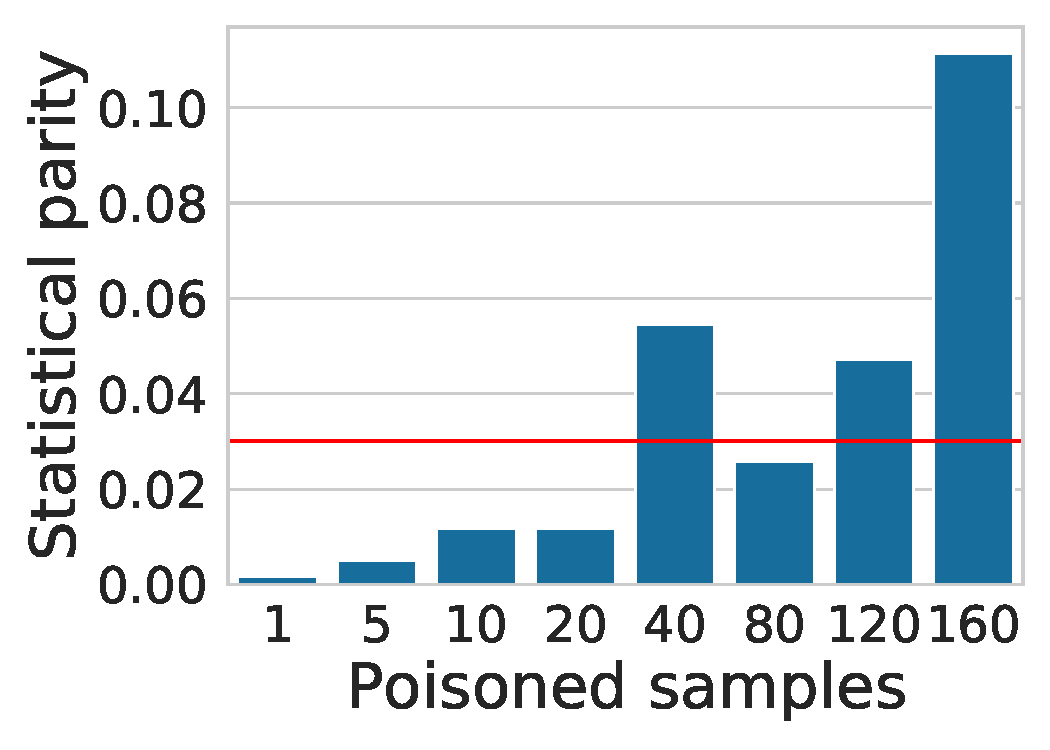
\includegraphics[scale=0.3]{figures/fairness/fvgm/stat_fairness_attack}}
	
	\caption[Verifying fairness attacks]{Verifying poisoning attack against fairness using {\fvgm}. The red line denotes the safety margin of the machine learning model against the attack.}\label{fvgm_fig:fairness_attacks}
\end{figure}


\paragraph{Verifying Fairness Attacks.}
We apply {\fvgm} in verifying a fairness poisoning-attack algorithm. This algorithm injects a small fraction of poisoned samples into the training data such that the classifier becomes relatively unfair~\cite{solans2020poisoning}. We apply this attack to add $\{1, 5, \dots, 160\}$ poisoned samples  and measure the corresponding disparate impact and statistical parity. In Figure~\ref{fvgm_fig:fairness_attacks},  {\fvgm} verifies that the disparate impact of the classifier decreases and statistical parity increases, i.e.\textit{ the classifier becomes more unfair},\textit{ as the number of poisoned samples increases}. Therefore, {\fvgm} shows the potential of being deployed in safety-critical applications to detect fairness attacks. For example, if we set $0.9$ as an acceptable threshold of disparate impact, {\fvgm} can raise an alarm once $160$ poisoned samples are added.


\iffalse
\begin{table}[!t]
	
	\centering
	\small
	\caption{Verification of fairness algorithms using {\fvgm}. Numbers in bold refer to fairness improvement. RW and OP refer to reweighing and optimized-preprocessing algorithms.  }\label{fvgm_tab:fair_algo_verification}
	\setlength{\tabcolsep}{.4em}
	
	\begin{tabular}{lllrrrrrrrrrrrrr}
		
		\toprule
		Dataset & Sensitive & Algo. & $ \Delta $ DI &  $ \Delta $ PCF & $ \Delta $ SP & $ \Delta $ EO\\
		\midrule
		
		
		\multirow{4}{*}{Adult}&\multirow{2}{*}{race}&RW&$ \textbf{0.53} $&$ \textbf{-0.06} $&$ \textbf{-0.06} $&$ \textbf{-0.02} $\\
		&&OP&$ \textbf{0.57} $&$ \textbf{-0.07} $&$ \textbf{-0.07} $&$ \textbf{-0.02} $\\
		\cmidrule{2-7}
		&\multirow{2}{*}{sex}&RW&$ \textbf{0.96} $&$ \textbf{-0.16} $&$ \textbf{-0.15} $&$ \textbf{-0.08} $\\
		&&OP&$ \textbf{0.43} $&$ \textbf{-0.08} $&$ \textbf{-0.08} $&$ 0.03 $\\
		
		\midrule
		\multirow{4}{*}{COMPAS}&\multirow{2}{*}{race}&RW&$ \textbf{0.13} $&$ \textbf{-0.07} $&$ \textbf{-0.07} $&$ \textbf{-0.06} $\\
		&&OP&$ \textbf{0.15} $&$ \textbf{-0.08} $&$ \textbf{-0.08} $&$ \textbf{-0.05} $\\
		\cmidrule{2-7}
		&\multirow{2}{*}{sex}&RW&$ \textbf{0.1} $&$ \textbf{-0.04} $&$ \textbf{-0.04} $&$ 0.04 $\\
		&&OP&$ \textbf{0.09} $&$ \textbf{-0.04} $&$ \textbf{-0.04} $&$ \textbf{-0.03} $\\
		
		\midrule
		\multirow{4}{*}{German}&\multirow{2}{*}{age}&RW&$ \textbf{0.52} $&$ \textbf{-0.53} $&$ \textbf{-0.52} $&$ \textbf{-0.47} $\\
		&&OP&$ \textbf{0.53} $&$ \textbf{-0.53} $&$ \textbf{-0.53} $&$ \textbf{-0.51} $\\
		\cmidrule{2-7}
		&\multirow{2}{*}{sex}&RW&$ -0.06 $&$ 0.06 $&$ 0.06 $&$ 0.02 $\\
		&&OP&$ -0.12 $&$ 0.12 $&$ 0.12 $&$ 0.07 $\\
		
		
		\bottomrule
	\end{tabular}
\end{table}
\fi




\paragraph{Fairness Influence Function (FIF): Tracing Sources of Unfairness.}
Another application of \fvgm{} as a fairness verifier is to quantify the effect of a subset of features on fairness. Thus, we define fairness influence function (FIF)  that computes the effect of a subset of non-sensitive features $\mathbf{S} \subseteq \nonsensitive$ on the probability of positive prediction of a classifier given a specific sensitive group $ \sensitive = \mathbf{a}$,
$
	\mathsf{FIF}(\mathbf{S}) \triangleq \Pr[\hat{Y} = 1 | \sensitive = \mathbf{a}, \mathcal{D}] - \Pr[\hat{Y} = 1 | \sensitive = \mathbf{a},  \mathcal{D}_{-\mathbf{S}}].
$
FIF allows us to explain the sources of unfairness in the classifier. In practice, we compute FIF of $\mathbf{S}$ by replacing the probability distribution of $\mathbf{S}$ with a uniformly random distribution, referred to as  $ \mathcal{D}_{-\mathbf{S}} $, and reporting differences in the conditional probability of positive prediction of the classifier. 

In Figure~\ref{fvgm_fig:influence function}, we compute FIF for all features in COMPAS dataset, separately for two sensitive groups: Female (`sex' $ = 1 $) and Male. This dataset concerns the likelihood of a person of re-offending crimes within the next two years. We first observe that the base values of the probability of positive prediction are different for the two groups ($ 0.46 $ vs $ 0.61 $ for Female and Male), thereby showing Male as more probable to re-offend crimes than Female. Moreover, FIF of the feature `age' is comparatively higher in magnitude for Male than Female. 
This implies that while deciding recidivism the algorithm assumes that Female individuals across different ages re-offend crimes with almost the same probability and the probability of re-offending for Male individuals highly depends on age. Thus, applying {\fvgm} to compute FIF provides us insights about sources of bias and thus, indicators to improve fairness.

\begin{figure}[t!]	
	\centering
	\vspace{-2ex}
	\subfloat{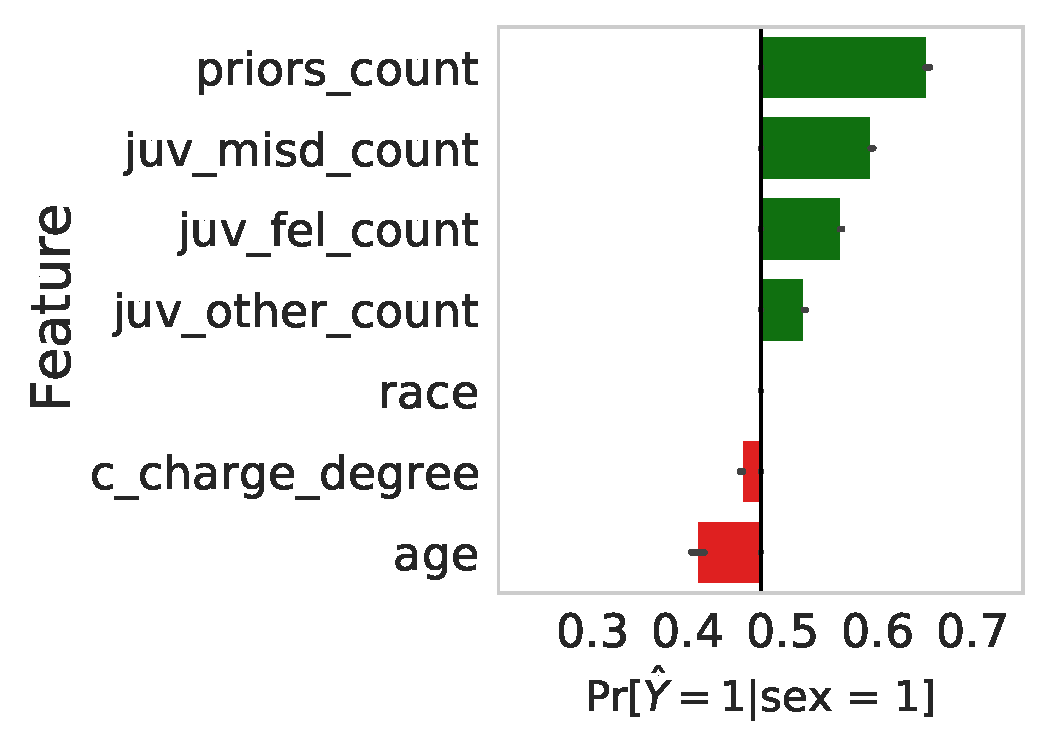
\includegraphics[scale=0.3]{figures/fairness/fvgm/dependency_exp_Learn-dependency_compas_lr_sex_1}}
	\subfloat{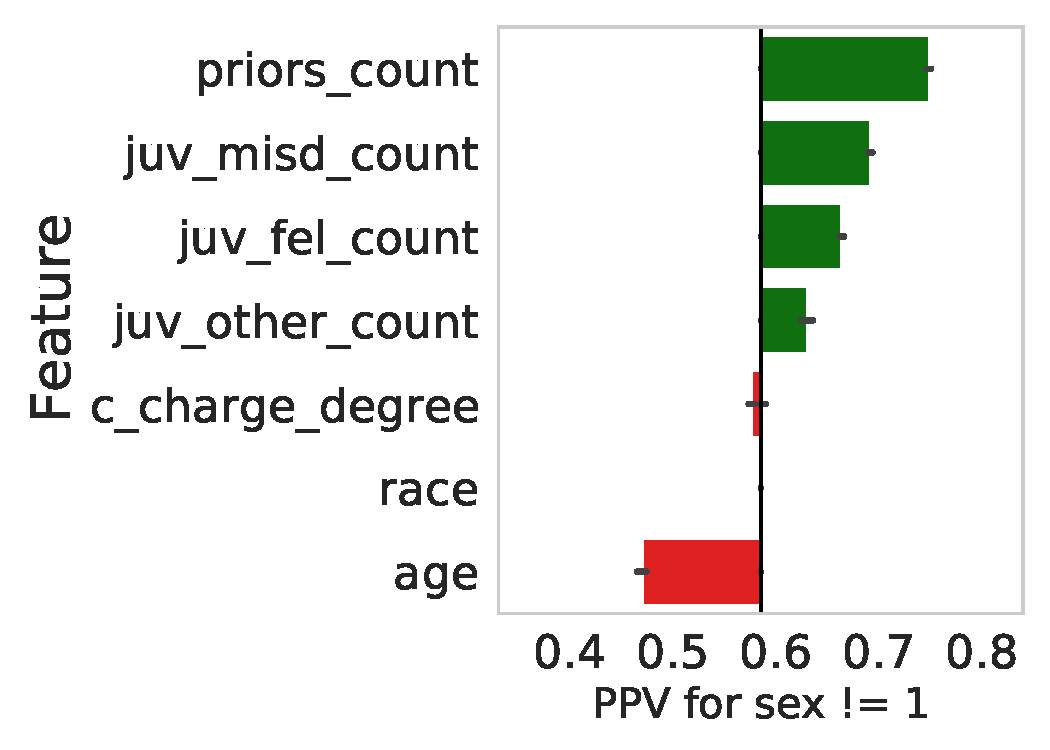
\includegraphics[scale=0.3]{figures/fairness/fvgm/dependency_exp_Learn-dependency_compas_lr_sex_0}}
	%\vspace{-0.5em}
%	\vspace{-2ex}
	\caption[FIF computation using {\fvgm}]{FIF computation for COMPAS dataset. For Female (left plot) and Male (right plot) individuals,  the influence of `age' decreases and the probability of positive prediction of the classifier increases  by different magnitudes.}\label{fvgm_fig:influence function}
%	\vspace{-2ex}
\end{figure}



